\lecture{5}{mon 20 sep 9:35}{Demand}
\section{Supply and Demand}
\begin{definition}
    Markets are \textbf{actual} or \textbf{nominal} place, where the forces of \textbf{demand} and \textbf{supply} operate. It is a place where \textbf{buyers} and \textbf{sellers} interact to trade \textbf{goods} or \textbf{services}. 
\end{definition}

In order to first understand supply and demand, its important to understand the relationship between price and quantity. Price is the amount of money paid for a good or service, and is commonly placed on the Y-axis on econ graphs. Quantity is the amount of a good/service that is purchased or provided, and is commonly placed on the X-axis on econ graphs. 

\begin{definition}
    Demand is a consumers' \textbf{willingness} and \textbf{ability} to buy at various price levels.
    \begin{itemize}
        \item Willingness: buyers want an item
        \item Ability: buyers have the financial resources to pay for an item
    \end{itemize}
\end{definition}

It is important to understand that demand is often a behavior, not a numerical amount. Demand has a inverse relationship between price and quantity. This leads to a downward sloping curve. With demand, it is important to understand the \textbf{Law of Demand}.
\begin{definition}
    Law of Demand is the idea that all other things equal, the quantity demanded of a good falls when the price of the good rises. 
\end{definition}

Now, it was mentioned that demand has a inverse relationship between price and quantity that leads to a downward sloping curve. There are 3 reasons why it has a downward sloping curve. 
\begin{itemize}
    \item Subsitution Effect
        \begin{itemize}
            \item When the price of peaches rises, consumers will substitute nectarines instead
        \end{itemize}
    \item Income Effect
        \begin{itemize}
            \item When something is expensive, money buys less
            \item When something is inexpensive, money buys more
        \end{itemize}
    \item Law of Diminishing Marginal Utility
        \begin{itemize}
            \item Each additional unit of an item purchases offers less marginal utility(happiness points)
            \item People will only buy more units if the price is lower, because of marginal decision making
        \end{itemize}
\end{itemize}
The net result of this is that if price goes up, the \textbf{Quantity Demanded} will go down, and the inverse is true. Make sure you understand the difference between \textbf{Quantity Demanded} and \textbf{Demand}.
\begin{definition}
    Quantity Demanded states that at a given price, how many units of X are demanded. QD will change as a result of a price change. 
\end{definition}

Demand is the number of units demanded at various prices, which differs from QD. Demand will change when something changes consumer's behaviors \textbf{at all price levels} (demand curve shifts).\\
\textbf{What can shift the Demand curve?}
\begin{itemize}
    \item \textbf{T}astes and Preferences
    \item \textbf{R}elated Goods
        \begin{itemize}
            \item Complements
            \item Substitutes
        \end{itemize}
    \item \textbf{I}ncome
        \begin{itemize}
            \item Normal Goods
            \item Inferior Goods
        \end{itemize}
    \item \textbf{P}opulation
    \item \textbf{E}xpectations
\end{itemize}
Quickly, lets define some of those terms:
\begin{description}
\item[Complements] Goods/services used along with each other, like Eggs and Bacon or Chips and Salsa
\item[Substitutes] Goods/services used instead of each other, like Butter and Margarine
\item[Normal Goods] When income rises, demand rises; When income falls, demand falls
\item[Inferior Goods] When income rises, demand falls; When income falls, demand rises
\end{description}

Changes in prices can help affect the demand curve for complements and substitutes. Lets say there is a sale on salsa, we can model the supply and demand on salsa and chips.  
\begin{figure}[H]
\begin{center}
\hspace*{-3cm}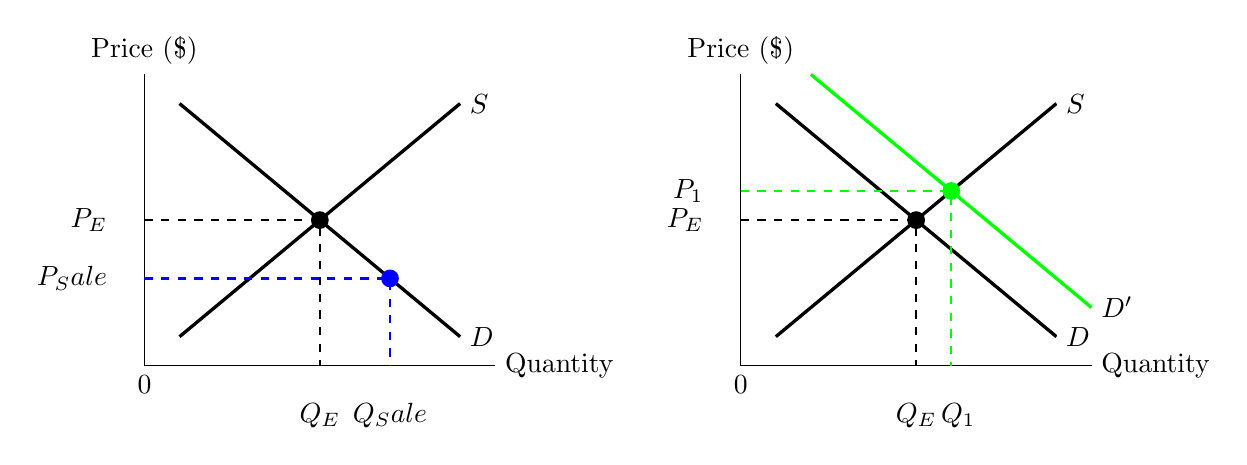
\begin{tikzpicture}
\begin{axis}[
% Insert parameters for Graph 1
scale = 0.65,
xmin = 0, xmax = 10,
ymin = 0, ymax = 10,
axis lines* = left,
xtick = {0}, ytick = \empty,
clip = false,
]
% Insert commands for Graph 1

% Supply and demand curves
\addplot[color = black, very thick] coordinates {(1, 9) (9, 1)};
\addplot[color = black, very thick] coordinates {(1, 1) (9, 9)};

% Dashed lines
\addplot[color = black, dashed, thick] coordinates {(0, 5) (5, 5) (5, 0)};
\addplot[color = blue, dashed, thick] coordinates {(0,3) (7,3) (7,0)};

% Coordinate points
\addplot[color = black, mark = *, only marks, mark size = 3pt] coordinates {(5, 5)};
\addplot[color = blue, mark = *, only marks, mark size = 3pt] coordinates {(7, 3)};

% Labels
\node [right] at (current axis.right of origin) {Quantity};
\node [above] at (current axis.above origin) {Price (\$)};
%\node [above = 5pt, fill = white, fill opacity = 0] at (5, 5) {$E$};
\node [left = 10pt] at (0, 5) {$P_E$};
\node [below = 10pt] at (5, 0) {$Q_E$};
%\node [above = 5pt, fill = white, fill opacity = 0] at (6, 4) {$E^\prime$};
\node [left = 10pt] at (0,3) {$P_Sale$};
\node [below = 10pt] at (7,0) { $Q_Sale$};
\node [right, fill = white] at (9, 1) {$D$};
\node [right, fill = white] at (9, 9) {$S$};
\end{axis}
\begin{axis}[
% Insert parameters for Graph 2
scale = 0.65,
xmin = 0, xmax = 10,
ymin = 0, ymax = 10,
axis lines* = left,
xtick = {0}, ytick = \empty,
clip = false,
shift = {(axis cs: 17, 0)},
]
% Insert commands for Graph 2
% Supply and demand curves
\addplot[color = black, very thick] coordinates {(1, 9) (9, 1)};
\addplot[color = black, very thick] coordinates {(1, 1) (9, 9)};
\addplot[color = green, very thick] coordinates {(2,10) (10,2)};

% Dashed lines
\addplot[color = black, dashed, thick] coordinates {(0, 5) (5, 5) (5, 0)};
\addplot[color = green, dashed, thick] coordinates {(0,6) (6,6) (6,0)};

% Coordinate points
\addplot[color = black, mark = *, only marks, mark size = 3pt] coordinates {(5, 5)};
\addplot[color = green, mark = *, only marks, mark size = 3pt] coordinates {(6,6)};
% Labels
\node [right] at (current axis.right of origin) {Quantity};
\node [above] at (current axis.above origin) {Price (\$)};
%\node [above = 5pt, fill = white] at (5, 5) {$E$};
\node [left = 10pt] at (0, 5) {$P_E$};
\node [below = 10pt] at (5, 0) {$Q_E$};
%\node [above = 5pt, fill = white] at (6, 4) {$E^\prime$};
\node [left = 10pt] at (0,6) {$P_1$};
\node [below = 10pt] at (6.2,0) { $Q_1$};
\node [right, fill = white] at (9, 1) {$D$};
\node [right, fill = white] at (9, 9) {$S$};
\node [right, fill = white] at (10,2) {$D^\prime$};
\end{axis}
\end{tikzpicture}\hspace*{-3cm}
\caption{Market for Salsa(L) and Chips(R)}
\label{fig:salsachips}
\end{center}
\end{figure}
The market for salsa will result in a shift \textbf{along} the demand curve, since price is the only thing that has changed. A lower price means more demand for the good, which is seen with the new equilibrium point. In the market for chips however, the entire demand curve will move to the right, since more people will want chips for the salsa they just bought.

Now, lets model the supply and demand for substitutes like butter and margarine.

\begin{figure}[!h]
\begin{center}
\hspace*{-3cm}\begin{tikzpicture}
\begin{axis}[
% Insert parameters for Graph 1
scale = 0.65,
xmin = 0, xmax = 10,
ymin = 0, ymax = 10,
axis lines* = left,
xtick = {0}, ytick = \empty,
clip = false,
]
% Insert commands for Graph 1

% Supply and demand curves
\addplot[color = black, very thick] coordinates {(1, 9) (9, 1)};
\addplot[color = black, very thick] coordinates {(1, 1) (9, 9)};

% Dashed lines
\addplot[color = black, dashed, thick] coordinates {(0, 5) (5, 5) (5, 0)};
\addplot[color = red, dashed, thick] coordinates {(0,3) (7,3) (7,0)};

% Coordinate points
\addplot[color = black, mark = *, only marks, mark size = 3pt] coordinates {(5, 5)};
\addplot[color = red, mark = *, only marks, mark size = 3pt] coordinates {(7, 3)};

% Labels
\node [right] at (current axis.right of origin) {Quantity};
\node [above] at (current axis.above origin) {Price (\$)};
%\node [above = 5pt, fill = white, fill opacity = 0] at (5, 5) {$E$};
\node [left = 10pt] at (0, 5) {$P_E$};
\node [below = 10pt] at (5, 0) {$Q_E$};
%\node [above = 5pt, fill = white, fill opacity = 0] at (6, 4) {$E^\prime$};
\node [left = 10pt] at (0,3) {$P_Sale$};
\node [below = 10pt] at (7,0) { $Q_Sale$};
\node [right, fill = white] at (9, 1) {$D$};
\node [right, fill = white] at (9, 9) {$S$};
\end{axis}
\begin{axis}[
% Insert parameters for Graph 2
scale = 0.65,
xmin = 0, xmax = 10,
ymin = 0, ymax = 10,
axis lines* = left,
xtick = {0}, ytick = \empty,
clip = false,
shift = {(axis cs: 17, 0)},
]
% Insert commands for Graph 2
% Supply and demand curves
\addplot[color = black, very thick] coordinates {(1, 9) (9, 1)};
\addplot[color = black, very thick] coordinates {(1, 1) (9, 9)};
\addplot[color = blue, very thick] coordinates {(1,6) (6,1)};

% Dashed lines
\addplot[color = black, dashed, thick] coordinates {(0, 5) (5, 5) (5, 0)};
\addplot[color = blue, dashed, thick] coordinates {(0,3.5) (3.5,3.5) (3.5,0)};

% Coordinate points
\addplot[color = black, mark = *, only marks, mark size = 3pt] coordinates {(5, 5)};
\addplot[color = blue, mark = *, only marks, mark size = 3pt] coordinates {(3.5,3.5)};
% Labels
\node [right] at (current axis.right of origin) {Quantity};
\node [above] at (current axis.above origin) {Price (\$)};
%\node [above = 5pt, fill = white] at (5, 5) {$E$};
\node [left = 10pt] at (0, 5) {$P_E$};
\node [below = 10pt] at (5, 0) {$Q_E$};
%\node [above = 5pt, fill = white] at (6, 4) {$E^\prime$};
\node [left = 10pt] at (0,6) {$P_1$};
\node [below = 10pt] at (6.2,0) { $Q_1$};
\node [right, fill = white] at (9, 1) {$D$};
\node [right, fill = white] at (9, 9) {$S$};
\node [right, fill = white] at (10,2) {$D^\prime$};
\draw[-{Triangle[length = 3mm, width = 2mm]}, blue, opacity = 0.3] (6, 3.5) to (4, 3.5);
\end{axis}
\end{tikzpicture}\hspace*{-3cm}
\caption{Market for Butter(L) and Margarine(R)}
\label{fig:salsachips}
\end{center}
\end{figure}
The market for butter will result in the same shift in demand, as a sale lowers price of a good, which increases \textbf{quantity demanded}. Since butter has become cheaper, and more desirable, butter will be substituted for margarine. Since less people are buying margarine, the demand curve shifts to the right, with less people willing to buy it at every price point.

Another one to watch out for is expectations, as consumers predicting what will happen will affect their demand. If consumers expects prices to rise in the future, then the demand will increase now. If they expect them to fall, demand decreases now because they will wait. The same analogy can be placed onto future income. If you expect your income to rise, you will start spending a bit more. The opposite is true as well. 
\begin{definition}
    A decrease in demand will cause the curve to shift left, a increase in demand will cause the curve to shift right. 
\end{definition}
